\documentclass[conference]{IEEEtran}
\IEEEoverridecommandlockouts
% The preceding line is only needed to identify funding in the first footnote. If that is unneeded, please comment it out.
\usepackage{cite}
\usepackage{amsmath,amssymb,amsfonts}
\usepackage{algorithmic}
\usepackage{graphicx}
\usepackage{textcomp}
\usepackage{xcolor}
\usepackage{tikz}
\usepackage{pgfplots}
%\usepackage[top=30pt,bottom=35pt,left=48pt,right=46pt]{geometry}
\def\BibTeX{{\rm B\kern-.05em{\sc i\kern-.025em b}\kern-.08em
    T\kern-.1667em\lower.7ex\hbox{E}\kern-.125emX}}
\begin{document}

\title{Report: Image Processing and Computer Vision 2018}

\author{
\IEEEauthorblockN{Florian Bauer}
\IEEEauthorblockA{\textit{School of Computer Science} \\
\textit{University of Bristol}\\
Bristol, UK\\
ya18048@bristol.ac.uk}
\and
\IEEEauthorblockN{Ruben Powar}
\IEEEauthorblockA{\textit{School of Computer Science} \\
\textit{University of Bristol}\\
Bristol, UK\\
TODO: wz18202@bristol.ac.uk}
}

\maketitle

\begin{abstract}TODO: Write an abstract or remove it later.
\end{abstract}

\section{Subtask 1}

The First Page of your Report (strict limit):\\
a) Annotate the test images to generate ground truth, then
test the face detector’s performance (with the given
parameters as provided by face.cpp) on five given example
images: dart4.jpg, dart5.jpg, dart13.jpg, dart14.jpg and
dart15.jpg. Produce the five result images with bounding
boxes drawn around detected face candidates and include
them in your report. \\
b) Calculate and note in your report the TPR (true positive
rate) for the images dart5.jpg and dart15.jpg, that is the
fraction of successfully detected faces out of all valid faces
in an image. Discuss in your team and briefly note in your
report 1) some practical difficulties in assessing the TPR
accurately, 2) why it is always possible to achieve a TPR of
100\% on any detection task, and 3) implement a small
piece of code to calculate the F1-score of your face
detection system accurately and meaningfully from
ground truth and a test run on any given test image set.

\subsection{Face detection}

\begin{figure}[ht!]
\centering
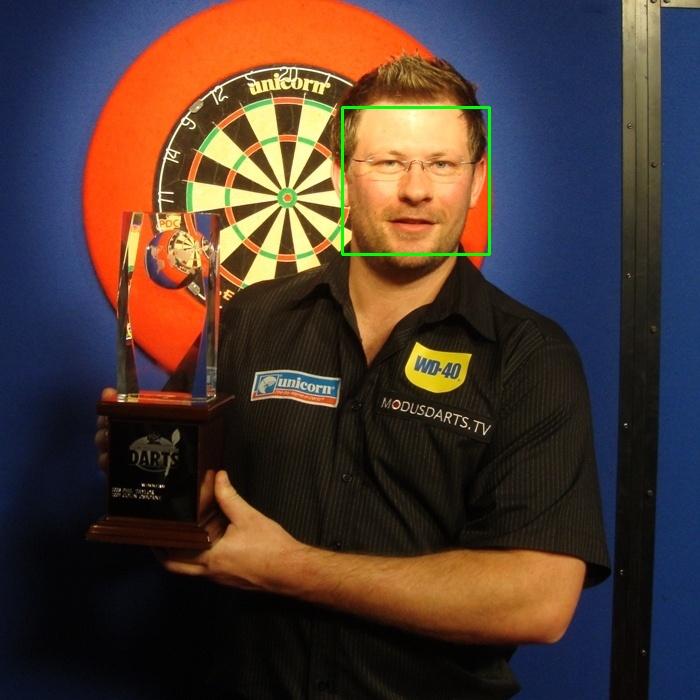
\includegraphics[width=60mm]{img/detected_dart4.jpg}
\caption{Image dart4.jpg \label{img_face_4}}
\end{figure}

\begin{figure}[ht!]
\centering
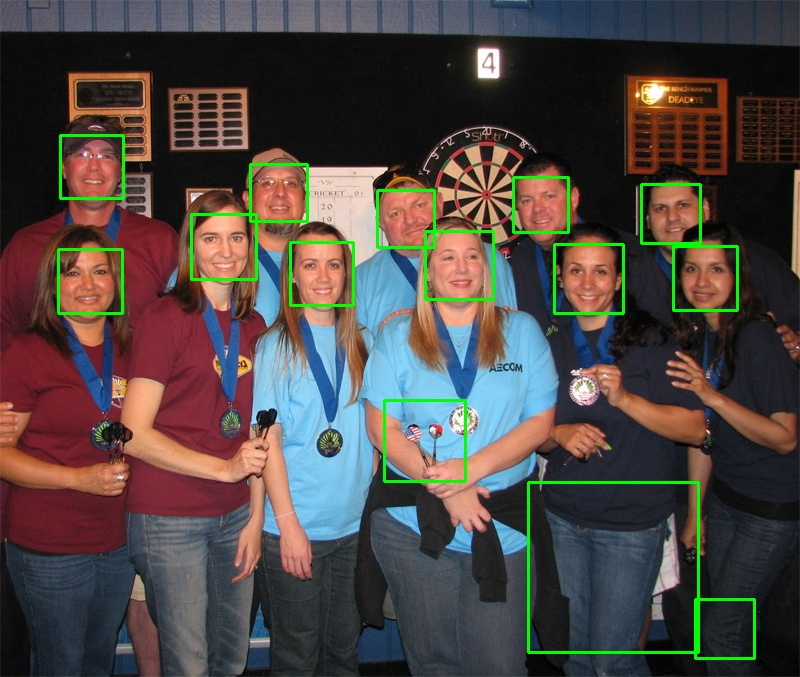
\includegraphics[width=60mm]{img/detected_dart5.jpg}
\caption{Image dart5.jpg \label{img_face_5}}
\end{figure}

\begin{figure}[ht!]
\centering
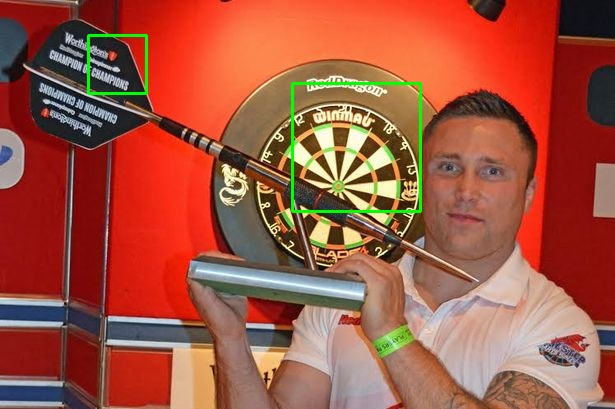
\includegraphics[width=60mm]{img/detected_dart13.jpg}
\caption{Image dart13.jpg \label{img_face_13}}
\end{figure}

\begin{figure}[ht!]
\centering
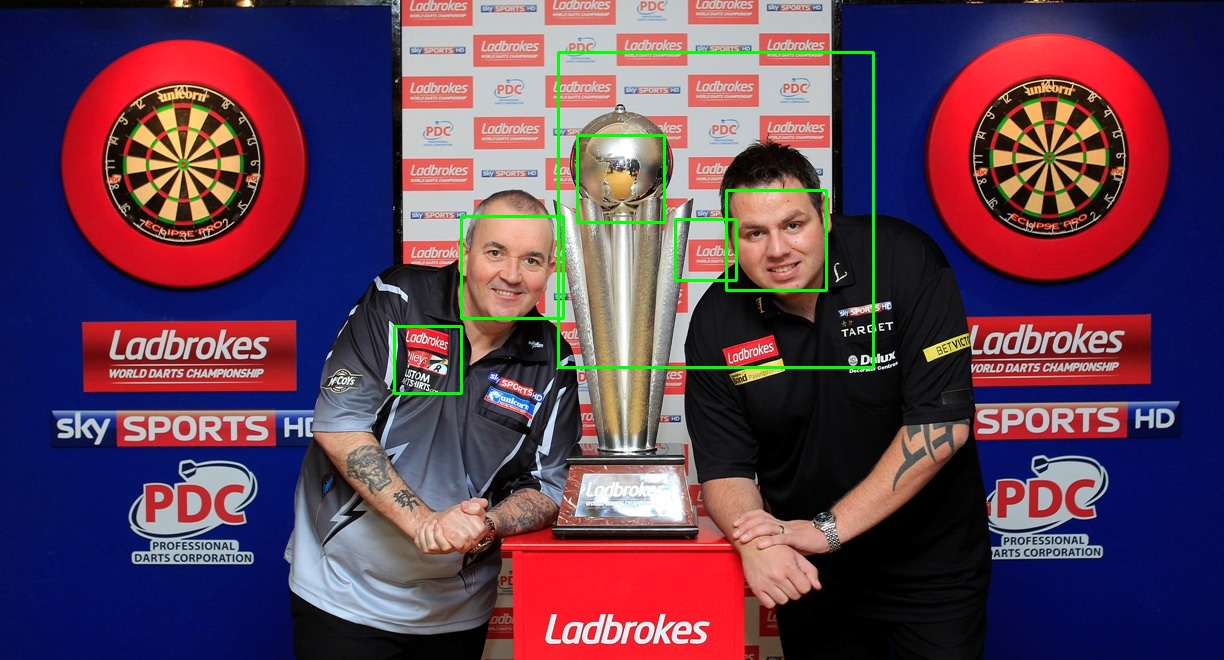
\includegraphics[width=60mm]{img/detected_dart14.jpg}
\caption{Image dart14.jpg \label{img_face_14}}
\end{figure}

\begin{figure}[ht!]
\centering
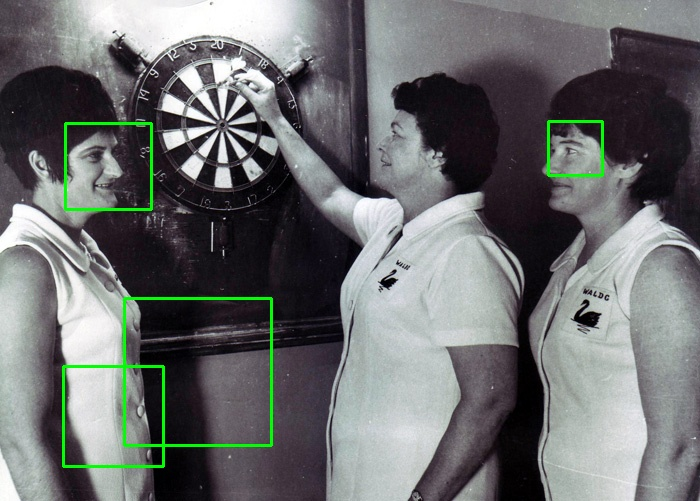
\includegraphics[width=60mm]{img/detected_dart15.jpg}
\caption{Image dart15.jpg \label{img_face_15}}
\end{figure}

\subsection{TPR calculation}

Calculating the true positive rate:
\[TPR = \frac{TP}{P} = \frac{TP}{TP+FN}\]
where :\\
$TPR$ = True positive rate \\
$TP$ = The number of cases correctly recognised \\
$P$ = The number of actual positive cases in the data\\
$FN$ = The number of false negatives, or the number of actual true cases not recognised\\

dart5.jpg TPR = 
\[\frac{11}{11+0} = 1 \therefore 100\%\]
dart15.jpg TPR = 
\[\frac{2}{2+1} = 0.\dot{6} \therefore 66.\dot{6}\%\]

It is always possible to achieve a TPR of 100\% on any detection as 

\newpage

\section{Subtask 2}

The Second Page of your Report (strict limit):\\
a) The training tool produces a strong classifier in stages. Per
stage the tool adds further features to the classifier and
prints the achieved TPR and FPR (false positive rate) for
that point on the training data (see Figure). Collate this
information into a scatter plot that plots TPR vs FPR on the
training data for the three different stages. Produce this
graph in your report and briefly interpret what it shows.\\
b) Test the dartboard detector’s performance on all given
example images. Produce the result images with bounding
boxes drawn around detected dartboard candidates and
include 4 of them in your report. In tabular form, calculate
the overall F1 score per image and the average across all
16 images. Briefly discuss the performance achieved and
compare it to the level of performance achieved in a).

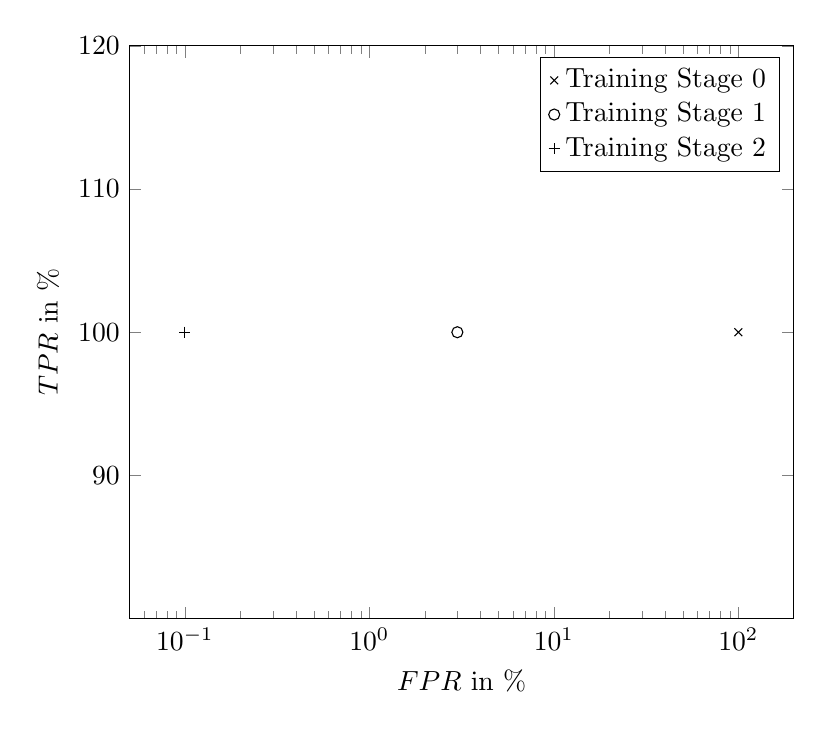
\begin{tikzpicture}

\pgfplotsset{
	scale only axis,
}

\begin{axis}[
    xmode=log,
xlabel=$FPR$ in \%,
ylabel=$TPR$ in \%,
]
\addplot[only marks, mark=x]
coordinates{ % plot 1 data set
	(100,100)
	% more points...
}; \label{training stage 0}
\addplot[only marks, mark=o]
coordinates{ % plot 1 data set
	(3,100)
	% more points...
}; \label{training stage 1}
\addplot[only marks, mark=+]
coordinates{ % plot 1 data set
	(0.1,100)
	% more points...
}; \label{training stage 2}

% plot 1 legend entry
\addlegendimage{/pgfplots/refstyle=plot_one}
\addlegendentry{Training Stage 0}
\addlegendentry{Training Stage 1}
\addlegendentry{Training Stage 2}
\end{axis}

\end{tikzpicture}

As training progresses from stage 0 to 2 we see that the \textit{true positive rate} (TPR) appears to remain constant. This is due to being parametrised with a minimum hit rate of 0.999, essentially ensuring that all dartboards are detected while the algorithm attempts to reduce the number of false positives. We can see that \textit{false positive rate} decreases at an exponential rate between each of the training stages.

\section{Subtask 3}

The Third Page of your Report (strict limit):\\
a) Show in your report for two of the given example dart
images which best exhibit the merit and limitations of your
implementation: 1) the thresholded gradient magnitude
image used as input to the Hough Transform, 2) a 2D
representation of the Hough Space, 3) the result images
showing final detections using bounding boxes.\\
b) Evaluate your detector on all of the example images.
Provide the F1-score of overall detection performance for
the set of example test images in a table. Document your
overall detection results (for instance by using
precision/recall measures) and briefly note in bullet points
the key merits and shortcomings of your implementation.\\
c) In a flow diagram, depict how you have combined
evidence from the Hough Transform and Viola-Jones
detector. In bullet points, explain briefly your rationale
behind the way you have combined evidence.

\section{Subtask 4}

The Forth Page of your Report (strict limit):\\
a) In bullet points, explain briefly your rationale behind
selecting the approach you have taken.\\
b) Visualize important aspects of your technique in two of
the given example dart images selected to best exhibit the
merit of your approach.\\
c) Evaluate your final detector on all of the example images,
show the improvements in F1-score. Document your
overall detection results and briefly note in bullet points
the key merits and shortcomings of your final
implementation.

\end{document}